\documentclass[border=5mm]{standalone}
\usepackage{pgfplots}
\pgfplotsset{compat=1.17}

\begin{document}
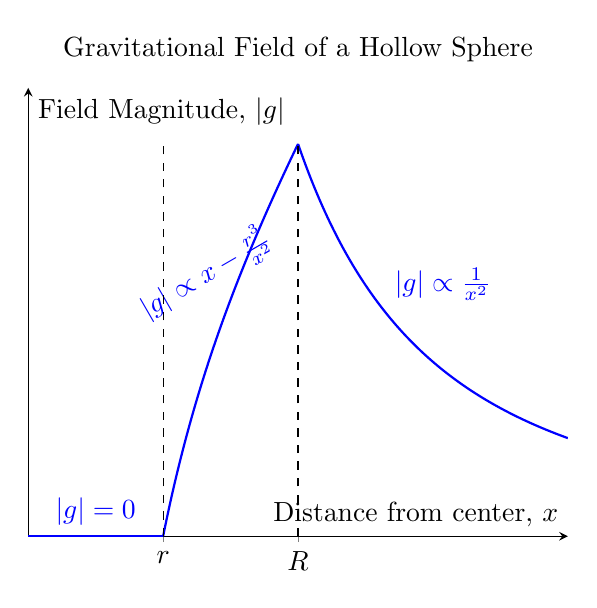
\begin{tikzpicture}
\begin{axis}[
    title={Gravitational Field of a Hollow Sphere},
    xlabel={Distance from center, $x$},
    ylabel={Field Magnitude, $|g|$},
    xmin=0, xmax=4,
    ymin=0, ymax=2,
    xtick={1,2},
    xticklabels={$r$, $R$},
    ytick=\empty,
    axis lines=middle,
    samples=100,
    domain=0:4,
    legend pos=north east,
    legend cell align={left}
]
    % Region 1: Inside the cavity (0 <= x < r)
    \addplot[blue, thick, domain=0:1] {0} node[pos=0.5, above] {$|g| = 0$};
    
    % Region 2: Within the material (r <= x <= R)
    \addplot[blue, thick, domain=1:2] {x - 1/x^2} node[pos=0.6, above, rotate=30, xshift=-2mm] {$|g| \propto x - \frac{r^3}{x^2}$};

    % Region 3: Outside the sphere (x > R)
    \addplot[blue, thick, domain=2:4] {7/x^2} node[pos=0.4, above right] {$|g| \propto \frac{1}{x^2}$};

    % Dashed lines to mark r and R
    \draw[dashed] (axis cs:1,0) -- (axis cs:1,1.75);
    \draw[dashed] (axis cs:2,0) -- (axis cs:2,1.75);
\end{axis}
\end{tikzpicture}
\end{document}